% CVPR 2025 Paper Template; see https://github.com/cvpr-org/author-kit

\documentclass[10pt,twocolumn,letterpaper,table]{article}

%%%%%%%%% PAPER TYPE  - PLEASE UPDATE FOR FINAL VERSION
% \usepackage{cvpr}              % To produce the CAMERA-READY version
% \usepackage[review]{cvpr}      % To produce the REVIEW version
\usepackage[pagenumbers]{cvpr} % To force page numbers, e.g. for an arXiv version
\usepackage{multirow}
\usepackage{xcolor}
% \usepackage{array}
% \usepackage[accsupp]{axessibility}

% Import additional packages in the preamble file, before hyperref
% \usepackage{amsmath}
% \usepackage{amssymb}
\usepackage{graphicx}
\usepackage{mathtools}
% \mathtoolsset{showonlyrefs}
\usepackage{amsfonts}
% \usepackage{amsthm,bm}
\usepackage{color}
% \usepackage{enumitem}
\usepackage{dsfont}
% \usepackage{pgfplots}
% \pgfplotsset{width=10cm,compat=1.9}
%  \usepackage{pifont}%http://ctan.org/pkg/pifont
\usepackage{thmtools} 
% \usepackage{thm-restate}
% \usepackage{sidecap}

\declaretheorem[name=Theorem]{thm}
\declaretheorem[name=Proposition]{prop}
\declaretheorem[name=Corollary]{cor}


\newcommand{\cmark}{\ding{51}}%
\newcommand{\xmark}{\ding{55}}%
\newcommand{\R}{\mathbb{R}}
\newcommand{\upmark}{\ding{218}}
\newcommand{\downmark}{\ding{216}}
\newcommand{\norm}[1]{\lVert#1\rVert}
\newcommand{\dotprod}[1]{\langle #1\rangle}
\newcommand{\E}{\mathbb{E}} 
\newcommand{\Et}[1]{\mathbf{E}_t\left[#1\right] } 
\newcommand{\Ev}[1]{\mathbf{E}_v\left[#1\right] } 
\newcommand{\EE}[2]{\mathbf{E}_{#1}\left[#2\right] } 
\newcommand{\Prb}[1]{\mathbf{P}\left[#1\right] }
\newcommand{\Tr}[1]{\mathrm{Tr}( #1)}
\newcommand{\Rea}[1]{\mathrm{Re}[ #1]}
\newcommand{\Ima}[1]{\mathrm{Im}[ #1]}
\newcommand{\eqdef}{\overset{\text{def}}{=}} 
\newcommand{\floor}[1]{\lfloor #1 \rfloor}
\newcommand{\Cov}[1]{\mathrm{Cov}\left[#1\right]}
\newcommand{\Var}[1]{\mathrm{Var}\left[#1\right]}
%\newcommand{\argmin}[1]{\underset{#1}{\text{argmin }}  } 
\newcommand{\breg}[2]{\mathcal{D}_{\Phi}\left(#1,#2\right) }
\newcommand{\xx}{\mathbf{x}}
\newcommand{\yy}{\mathbf{y}}
\newcommand{\zz}{\mathbf{z}}
\newcommand{\hmu}{\hat{\mu}}
\renewcommand{\phi}{\varphi}

%\usepackage{algorithm}
%\usepackage[noend]{algpseudocode}

\newcommand{\carles}[1]{{\color{red}{\bf[Carles:} #1{\bf]}}}
\newcommand{\ricky}[1]{{\color{magenta}{\bf[Ricky:} #1{\bf]}}}
\newcommand{\brian}[1]{{\color{orange}{\bf[Brian:} #1{\bf]}}}

% \newcommand{\carles}[1]{}
% \newcommand{\ricky}[1]{}
% \newcommand{\brian}[1]{}

\setlength{\parskip}{0.5em}
\setlength\parindent{0pt}

\graphicspath {{figures/}}

\newcommand{\N}{\mathbb{N}}
\newcommand{\Ff}{\mathcal{F}}
\newcommand{\Gg}{\mathcal{G}}
\usepackage{hyperref}
\usepackage{caption}
\usepackage[super]{nth}
\delimitershortfall-1sp

\newtheorem{lemma}{Lemma}
\newtheorem{definition}{Definition}
\newtheorem{theorem}{Theorem}
\newtheorem{note}{Note}
\newtheorem{assumption}{Assumption}
\newtheorem{proposition}{Proposition}
\newtheorem{example}{Example}
\newtheorem{remark}{Remark}
\newtheorem{corollary}{Corollary}
\newtheorem{observation}{Observation}
% \newtheorem{algorithm}{Algorithm}
\usepackage{subcaption}
%\newcommand{\corollaryautorefname}{Corollary}

\DeclareMathOperator*{\argmin}{argmin}
\DeclareMathOperator*{\argmax}{argmax}

\DeclarePairedDelimiter\abs{\lvert}{\rvert}

\renewcommand{\sectionautorefname}{Sec.}
\renewcommand{\subsectionautorefname}{Subsec.}
\renewcommand{\appendixautorefname}{App.}
\renewcommand{\theoremautorefname}{Thm.}
\renewcommand{\propositionautorefname}{Prop.}
\renewcommand{\corollaryautorefname}{Cor.}
% \renewcommand(\algorithmautorefname}{Alg.}

\newenvironment{talign*}
 {\let\displaystyle\textstyle\csname align*\endcsname}
 {\endalign}
\newenvironment{talign}
 {\let\displaystyle\textstyle\csname align\endcsname}
 {\endalign}

\makeatletter
\renewcommand{\thealgorithm}{\arabic{algorithm}}
% \@addtoreset{algorithm}{chapter}  % Remove or modify this line if you do not want to reset with chapters
\makeatother

\makeatletter
\DeclareRobustCommand{\cev}[1]{%
  {\mathpalette\do@cev{#1}}%
}
\newcommand{\do@cev}[2]{%
  \vbox{\offinterlineskip
    \sbox\z@{$\m@th#1 x$}%
    \ialign{##\cr
      \hidewidth\reflectbox{$\m@th#1\vec{}\mkern4mu$}\hidewidth\cr
      \noalign{\kern-\ht\z@}
      $\m@th#1#2$\cr
    }%
  }%
}
\makeatother

\definecolor{mygray}{gray}{0.95}
\newcommand{\greybox}[1]{
\vspace{-0.9em}
\begin{center}			% Centering minipage
\vspace{-0.5em}
\colorbox{mygray} {		% Set's the color of minipage
\begin{minipage}{0.987\linewidth} 	% Starts minipage
\centering
\vspace{-0.8em}
{#1}
\end{minipage}}			% End minipage
\end{center}
\vspace{-0.5em}
}

% It is strongly recommended to use hyperref, especially for the review version.
% hyperref with option pagebackref eases the reviewers' job.
% Please disable hyperref *only* if you encounter grave issues, 
% e.g. with the file validation for the camera-ready version.
%
% If you comment hyperref and then uncomment it, you should delete *.aux before re-running LaTeX.
% (Or just hit 'q' on the first LaTeX run, let it finish, and you should be clear).
\definecolor{cvprblue}{rgb}{0.21,0.49,0.74}
\usepackage[pagebackref,breaklinks,colorlinks,allcolors=cvprblue]{hyperref}

%%%%%%%%% PAPER ID  - PLEASE UPDATE
% \def\paperID{7929} % *** Enter the Paper ID here
% \def\confName{CVPR}
% \def\confYear{2025}

\renewcommand{\thefootnote}{}
\newcommand{\name}{STAR}
% \newcommand{\name}{$\mathtt{STAR}$}
%%%%%%%%% TITLE - PLEASE UPDATE
\title{STAR: Spatial-Temporal Augmentation with Text-to-Video Models\\ for Real-World Video Super-Resolution}

%%%%%%%%% AUTHORS - PLEASE UPDATE
\author{
  Rui Xie$^{1*}$, \hspace{0.2cm}
  Yinhong Liu$^{1*}$, \hspace{0.2cm}
  Penghao Zhou$^2$, \hspace{0.2cm}
  Chen Zhao$^1$, \hspace{0.2cm}
  Jun Zhou$^3$ \\
  Kai Zhang$^1$, \hspace{0.2cm}
  Zhenyu Zhang$^1$, \hspace{0.2cm}
  Jian Yang$^{1}$, \hspace{0.2cm}
  Zhenheng Yang$^2$, \hspace{0.2cm}
  Ying Tai$^{1\dagger}$ \\
  $^1$Nanjing University, \hspace{0.2cm}
  $^2$ByteDance, \hspace{0.2cm}
  $^3$Southwest University \\
  {\small \url{https://nju-pcalab.github.io/projects/STAR}}
}


\begin{document}
% \maketitle

\twocolumn[{
\renewcommand\twocolumn[1][]{#1}
\maketitle
\begin{center}
    \captionsetup{type=figure}
    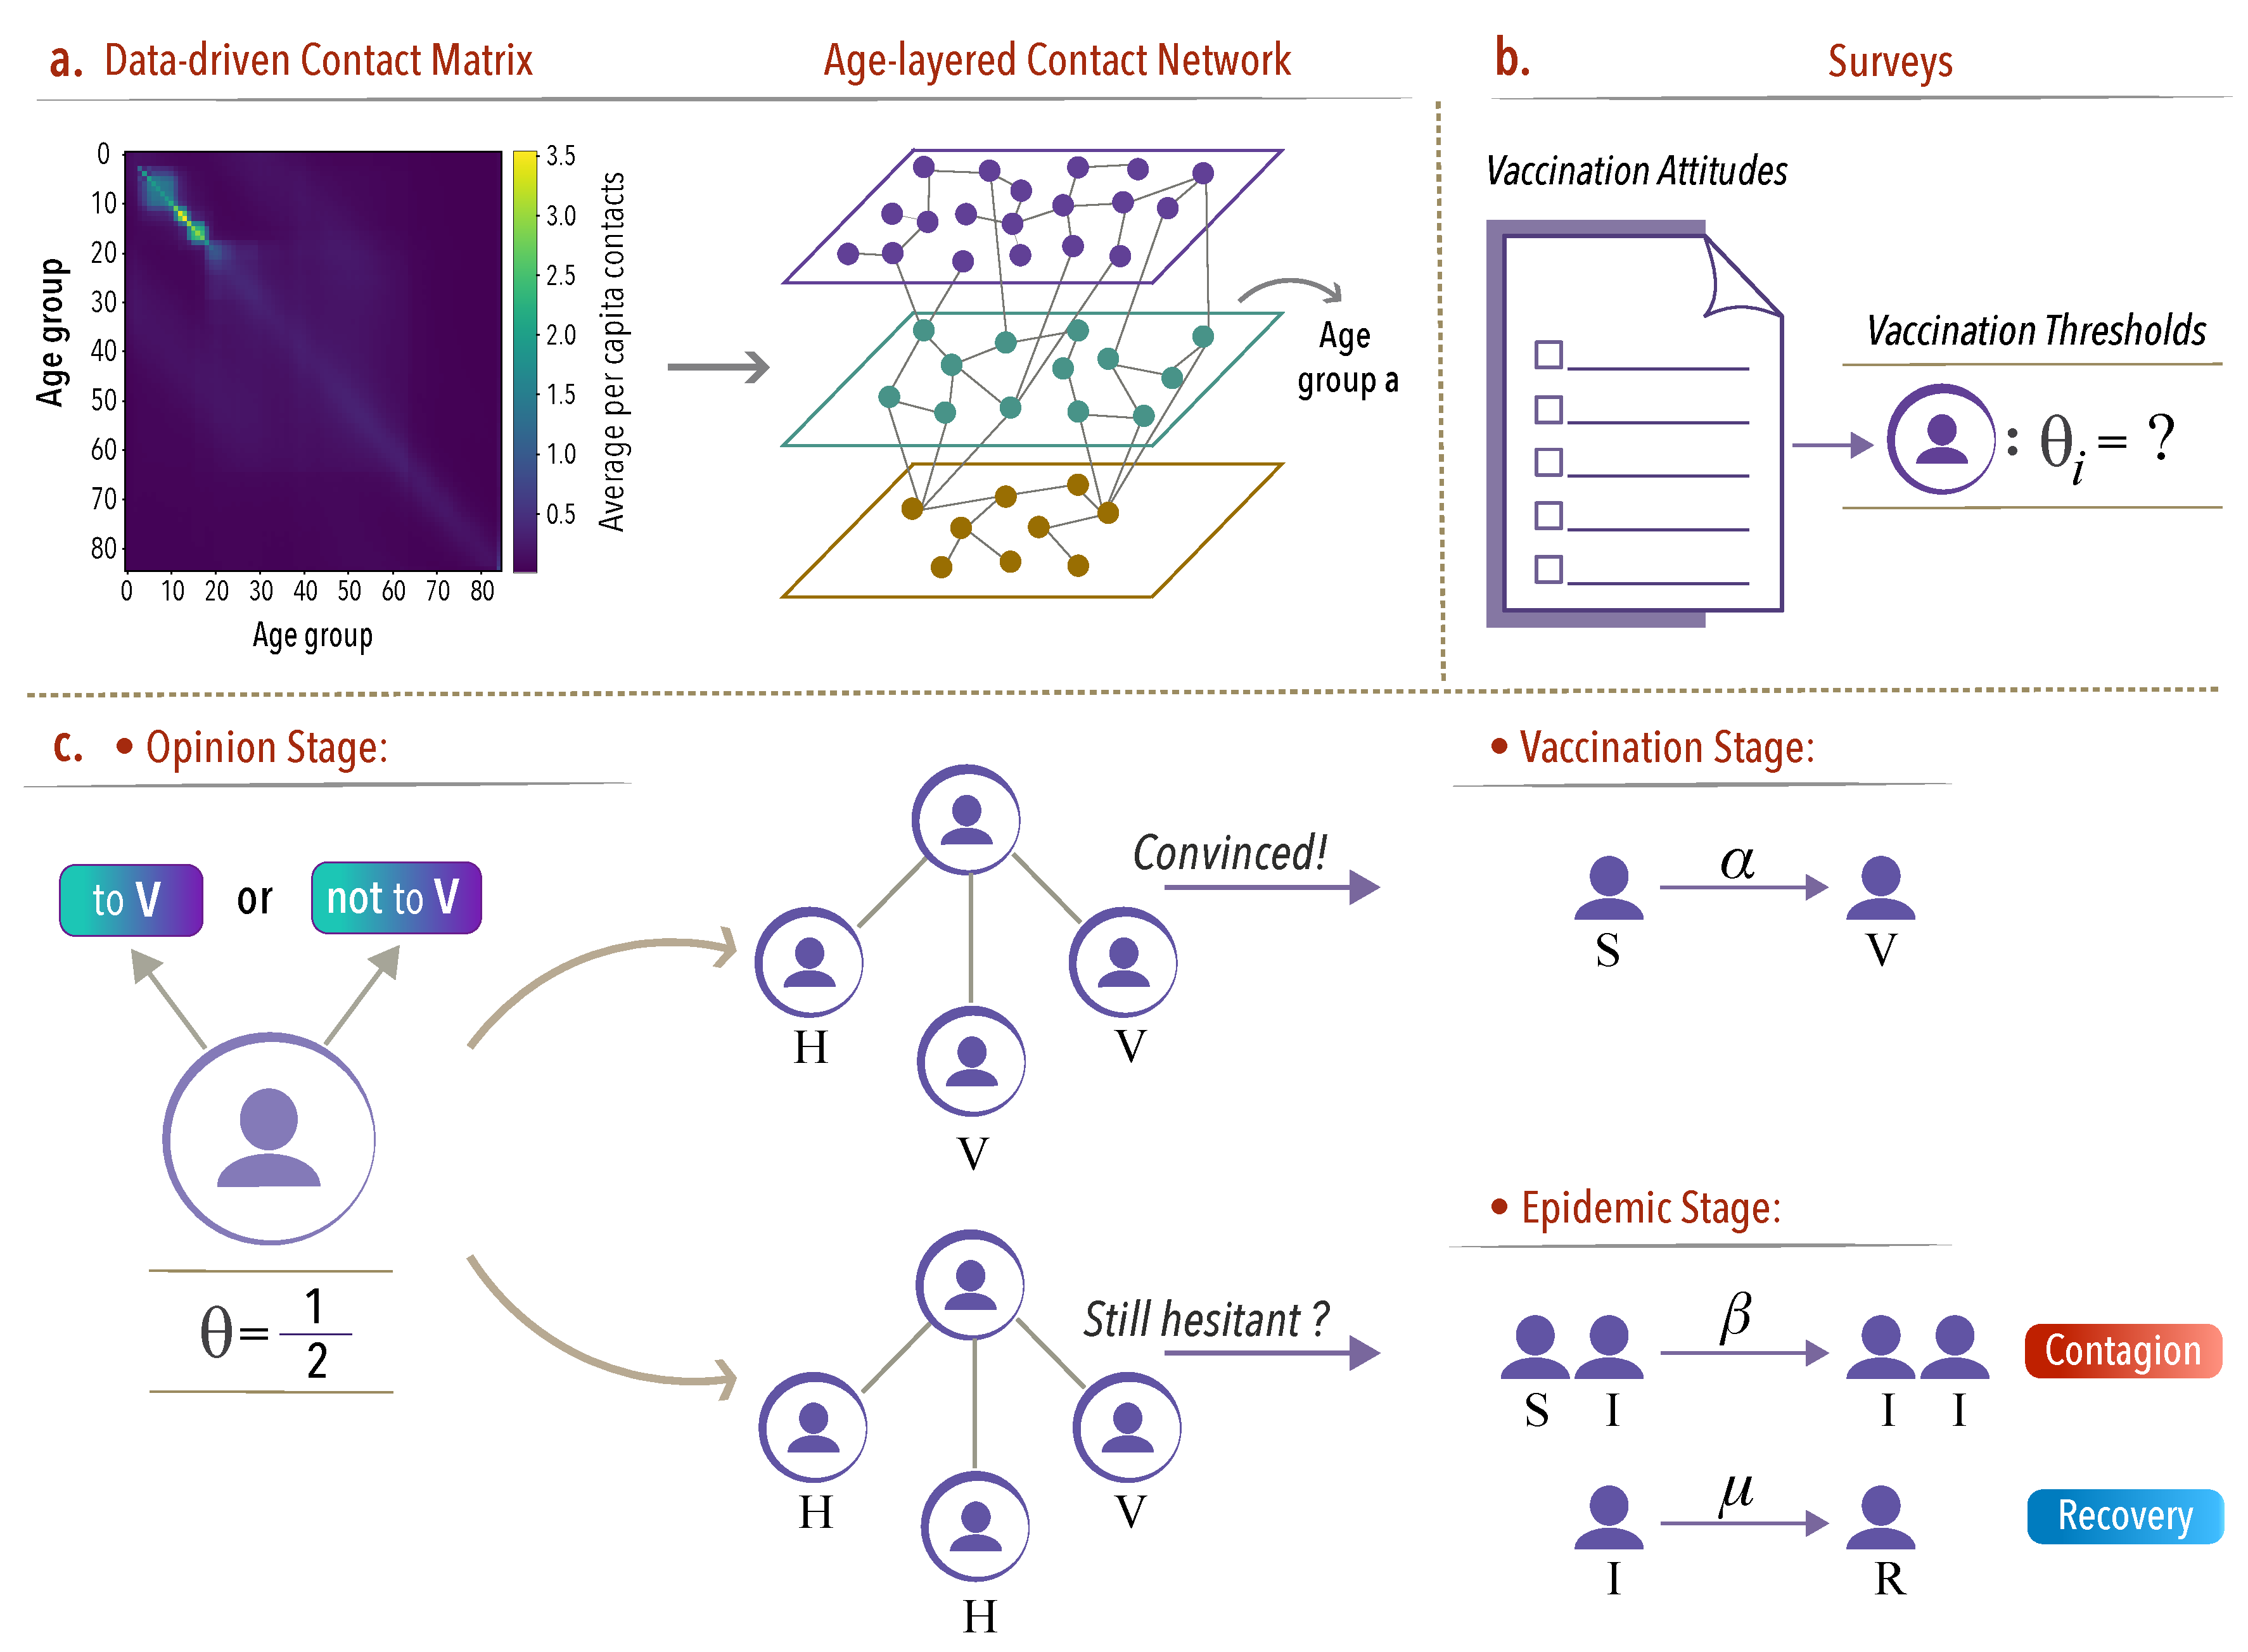
\includegraphics[width=\textwidth]{figure/figure1.pdf} \vspace{-6mm}
    \captionof{figure}{Visualization comparisons on both real-world and synthetic low-resolution videos. 
    Compared to the state-of-the-art VSR models~\cite{zhang2024realviformer,zhou2024upscale}, our results demonstrate more natural facial details and better structure of the text. 
    \textbf{(Zoom-in for best view)}}
    \label{teaser}
\end{center}
}]

\begin{abstract}
We introduce Causal Diffusion as the autoregressive (AR) counterpart of Diffusion models. It is a next-token(s) forecasting framework that is friendly to both discrete and continuous modalities and compatible with existing next-token prediction models like LLaMA and GPT. While recent works attempt to combine diffusion with AR models, we show that introducing sequential factorization to a diffusion model can substantially improve its performance and enables a smooth transition between AR and diffusion generation modes. Hence, we propose \textbf{CausalFusion} - a decoder-only transformer that dual-factorizes data across sequential tokens and diffusion noise levels, leading to state-of-the-art results on the ImageNet generation benchmark while also enjoying the AR advantage of generating an arbitrary number of tokens for in-context reasoning. We further demonstrate CausalFusion's multimodal capabilities through a joint image generation and captioning model, and showcase CausalFusion's ability for zero-shot in-context image manipulations. We hope that this work could provide the community with a fresh perspective on training multimodal models over discrete and continuous data.
\end{abstract}
\vspace{-10pt}
\section{Introduction}
\label{sec:intro}
Autoregressive (AR) and diffusion models are two powerful paradigms for data distribution modeling. AR models, also known as the next token prediction approach, dominate language modeling and are considered central to the success of large language models (LLMs)~\cite{gpt1,gpt2,gpt3,llama1,llama2,llama3}. On the other hand, diffusion models~\cite{ddpm,dit,adm,edm}, or score-based generative models~\cite{songscore,lipman2023flow}, have emerged as the leading approach for visual generation, driving unprecedented progress in the era of visual content generation~\cite{sora,rombach2022high,li2023scaling}. 

\begin{figure}[t]
    \centering
    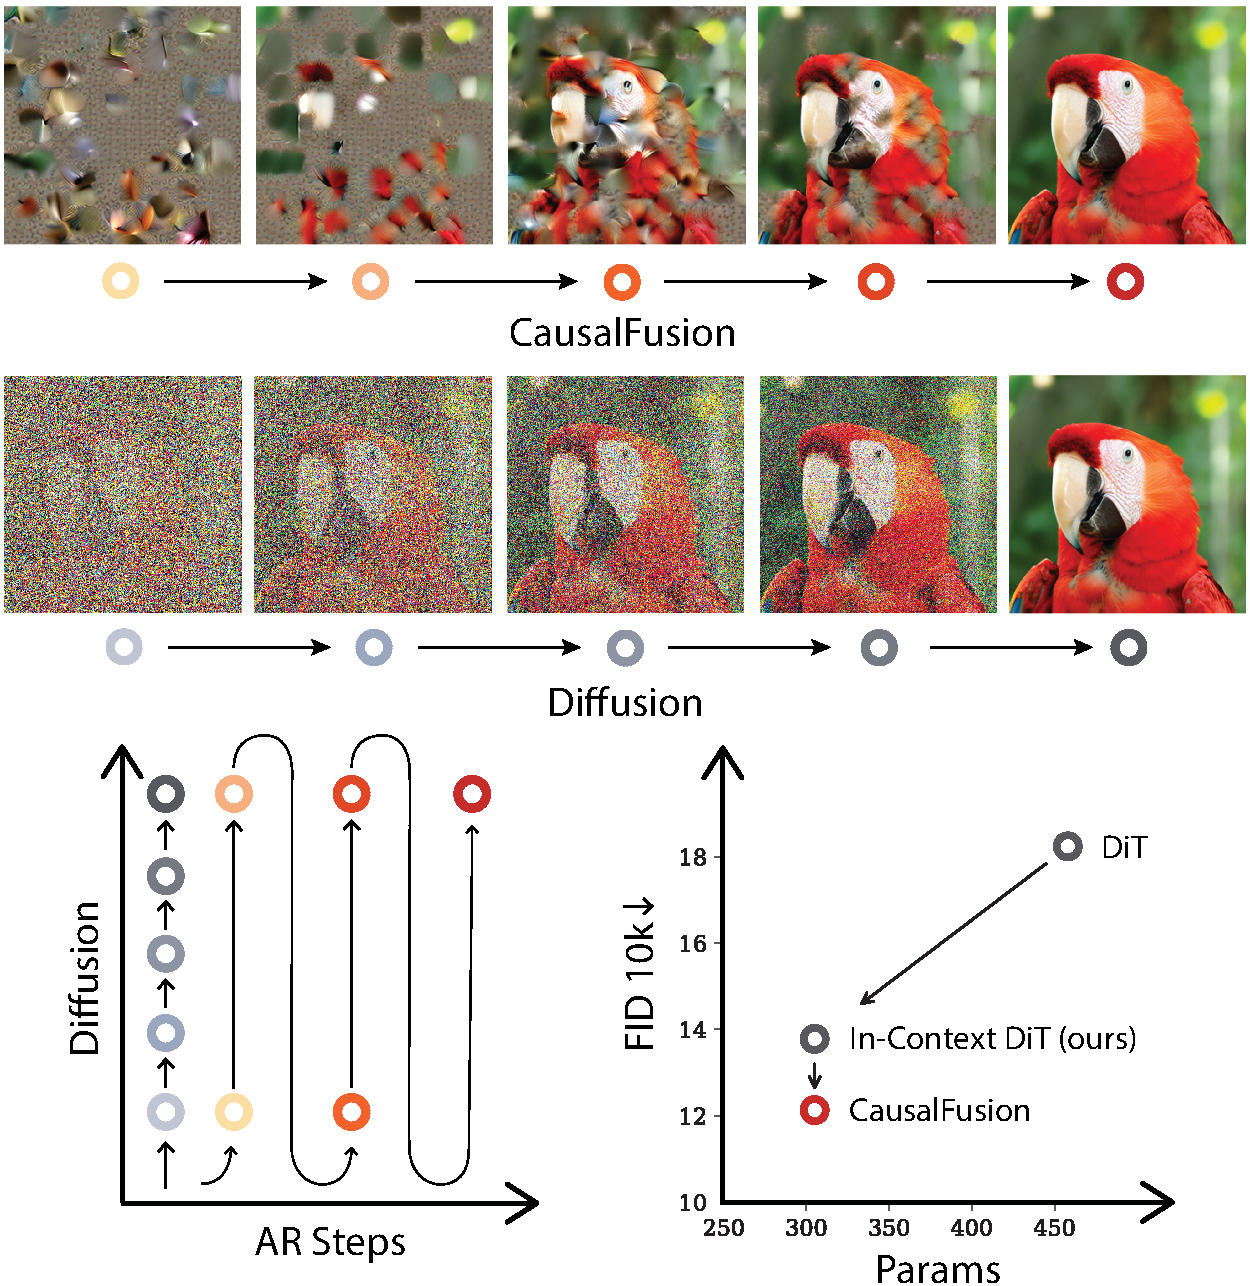
\includegraphics[width=1.0\textwidth,height=1.0\textwidth]{figs/casualfusion-teaser-v6.pdf} 
    \vspace*{-6mm}
    \caption{
    \textbf{Illustration of Dual-Factorization}. The arrow line indicates CausalFusion's generation path, moving from one state to the next by jointly generating along the sequential and noise-level dimension at each step. 
    Compared to DiT, our In-context DiT substantially improves results with fewer parameters. CausalFusion further enhances performance without changing the architecture or parameter count. Results were trained on IN1K for 240 epochs. CausalFusion adopts arbitrary AR steps for image generation, but each step only diffuses partial tokens, resulting in similar (or slightly lower) computational complexity.
    \vspace{-10pt}
    }
    \label{fig:dual-factorization}
\end{figure}


\begin{figure*}[t]
  \centering
  \begin{subfigure}{1.0\linewidth}
    \centering
    \includegraphics[width=\linewidth]{figs/figure2.pdf}
    \caption{Samples generated by CausalFusion-XL/2, ImageNet 512$\times$512, 800 epoch, DDPM 250 steps, CFG=4.0}
  \end{subfigure}
  \begin{subfigure}{1.0\linewidth}
    \centering
    \includegraphics[width=\linewidth]{figs/edit.pdf}
    \caption{\textbf{Zero-shot image editing} results generated by CausalFusion-XL/2, ImageNet 512$\times$512, 800 epoch. We first generate the original image (those on the left), then mask out its centre region, top-half, or bottom-half, and regenerate the image with new class conditions. Details are discussed in Sec \ref{sec:system}.}
  \end{subfigure}
  \caption{\textbf{Visualization results}. All samples are generated by models trained only on \textbf{ImageNet-1K class-conditional generation} task, demonstrating CausalFusion's zero-shot image manipulation ability. See more visualization results in Appendix~\ref{appendix:secD}.
  \vspace{-12pt}
  }
  \vspace{-6pt}
  \label{fig:vis1}
\end{figure*}

The intrinsic distinction between AR and diffusion models lies in their approach to data distribution factorization. AR models treat data as an ordered sequence, factorizing it along the sequential axis, where the probability of each token is conditioned on all preceding tokens. This factorization enables the AR paradigm to generalize effectively and efficiently across arbitrary number of tokens, making it well-suited for long-sequence reasoning and in-context generation. In contrast, diffusion models factorize data along the noise-level axis, where the tokens at each step are a refined (denoised) version of themselves from the previous step. As a result, the diffusion paradigm is generalizable to arbitrary number of data refinement steps, enabling iterative quality improvement with scaled inference compute. While AR and diffusion models each excel within their respective domains, their distinct factorization approaches reveal complementary potential. Although recent studies~\cite{transfusion,monoformer,dart} have attempted to integrate AR and diffusion within a single model, they typically treat these paradigms as separate modes, missing the potential benefits of jointly exploring them within a 2-D factorization plane.

To this end, we introduce \textbf{CausalFusion}, a flexible framework that integrates both sequential and noise-level data factorization to unify their advantages. The degree of factorization along these two axes—namely, the AR step and diffusion step—is adjustable, enabling {CausalFusion} to revert seamlessly to the traditional AR or diffusion paradigms at either extreme. To enhance its generality, CausalFusion is designed to predict \textit{any} number of tokens at \textit{any} AR step, with \textit{any} pre-defined sequence order and \textit{any} level of inference compute, thereby minimizing the inductive biases presented in existing generative models. As shown in Figure~\ref{fig:dual-factorization}, this approach provides a broad spectrum between the AR and diffusion paradigms, allowing smooth interpolation within two endpoints during both training and inference. 
Specifically, we explore CausalFusion in image generation and multimodal generation scenarios, where we observe that the level of training difficulties significantly influences the overall effectiveness of CausalFusion.

\textbf{Difficulties of generative tasks in CausalFusion:} Both AR and diffusion paradigms present unique challenges based on difficulties of their specific generative stages. In diffusion models, the effectiveness of training depends heavily on proper loss weighting across noise levels~\cite{ddpm,minsnr}, as higher noise levels are more difficult and usually provide more valuable signals than lower noise levels. Similarly, AR models are susceptible to error accumulation~\cite{bengio2015scheduled} as early-stage predictions are made with limited visible context, making them more error-prone. Optimizing CausalFusion thus requires balancing across these varying task difficulties to optimize training signal impact and ensure sufficient exploration across the entire factorization plane.

In this paper, we formally examine the difficulties of generative tasks within CausalFusion. We show that, in addition to the noise levels in diffusion and the amount of visible context in AR, the total number of AR steps, which controls the interpolation between AR and diffusion, also plays a critical role in shaping training difficulties. Driven by these factors, we develop a scalable and versatile model based on the CausalFusion framework. Starting from the DiT architecture~\cite{dit}, we gradually convert it into a decoder-only transformer compatible with existing AR models like GPT~\cite{gpt1,gpt2,gpt3} and LLaMA~\cite{llama1,llama2,llama3}. We provide insights on how to appropriately choose the number of AR steps during the training of CausalFusion models, and further introduce loss weighing along both the diffusion and AR axis to balance the impact of different generative stages. As shown in Figure~\ref{fig:dual-factorization} and ~\ref{fig:vis1}, our model achieves state-of-the-art performance on the ImageNet class-conditional generation benchmark, significantly outperforming DiT~\cite{dit} and enabling zero-shot image manipulations due to its AR nature. When pretraining on both text-to-image and image-to-text tasks, our model surpasses forced-fusion frameworks such as TransFusion~\cite{transfusion}, demonstrating the versatility of our CausalFusion framework.


We highlight our main contribution below:
\begin{itemize}
\item  We propose CausalFusion as the AR counterpart to DiT, achieving state-of-the-art results and enabling the unlimited token generation for in-context reasoning.
\item  We systematically study CausalFusion on the dual-factorization plane and identify key factors that improve the effectiveness of CausalFusion models.
\item  Compared with recent studies~\cite{transfusion}, CausalFusion enables a smooth, cohesive integration with language modeling for cross-modal generation and reasoning.
\end{itemize} 

\section{Related Work}
\label{sec:related work}

\begin{figure*}[t]
    \centering
    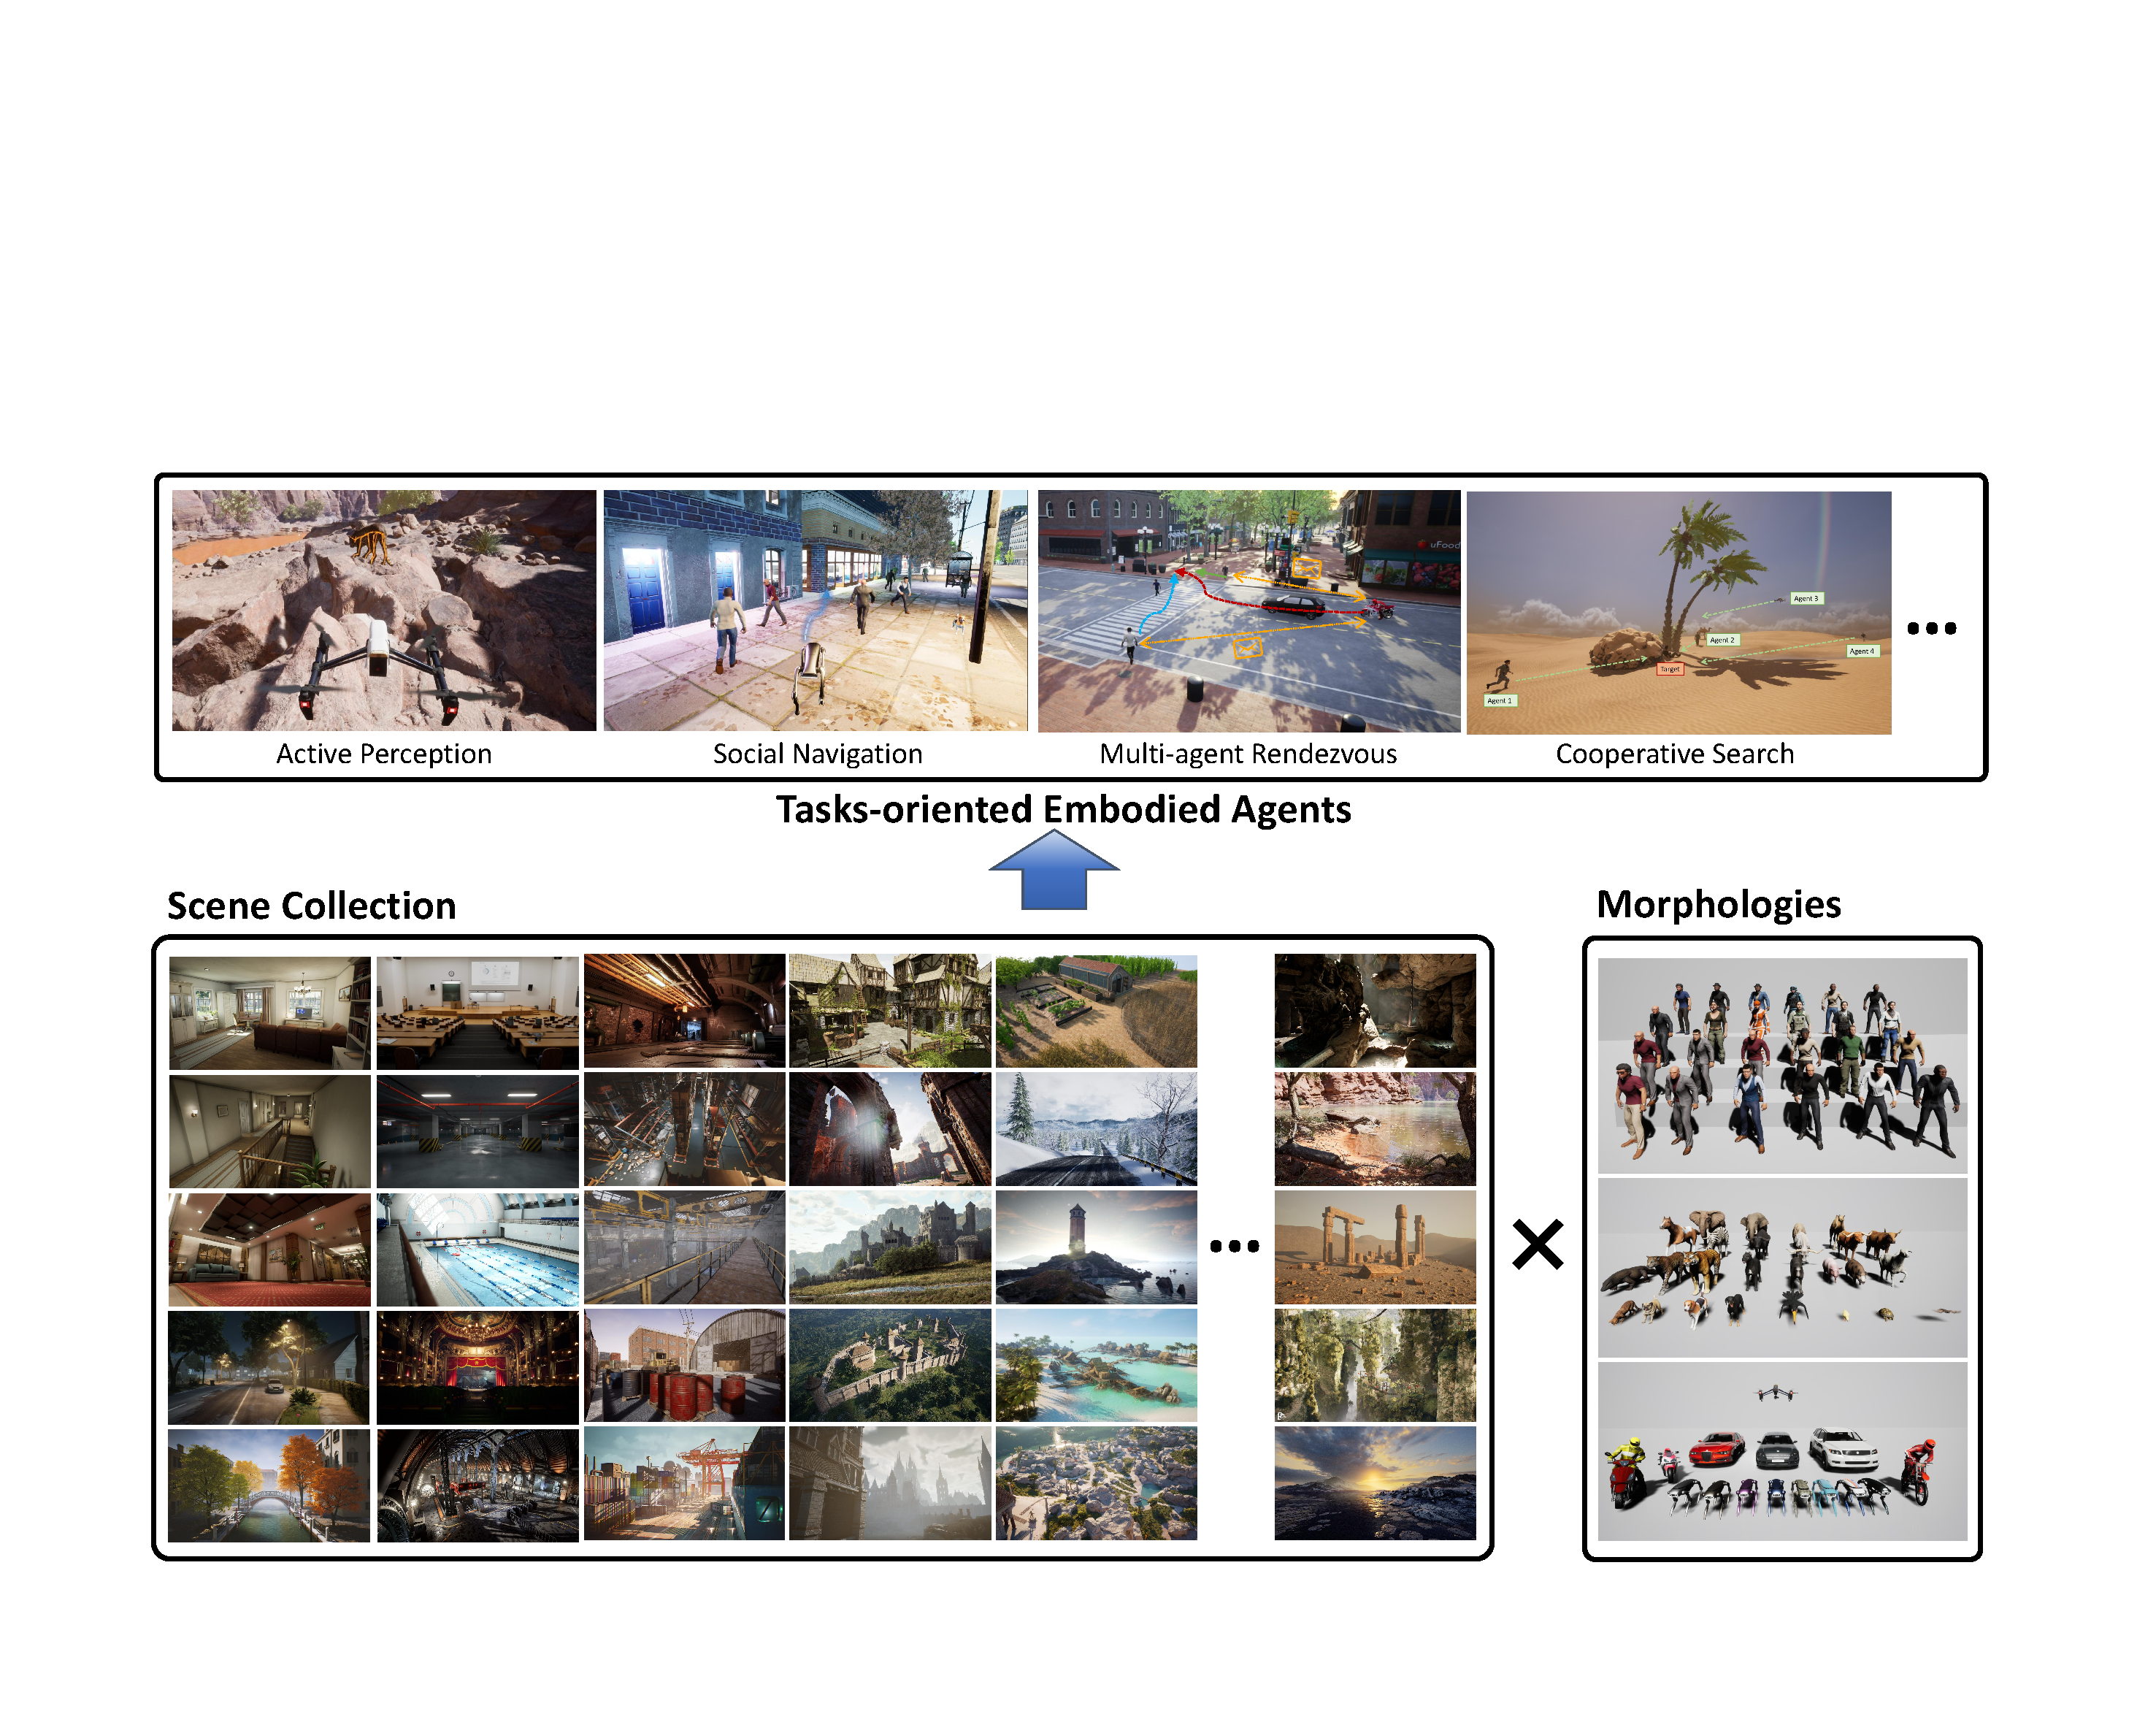
\includegraphics[width=1\linewidth]{figure/overview.pdf}\vspace{-2mm}
    \caption{Overview of the proposed~\name.}
    \label{fig:overview}
\end{figure*}

% \textbf{Video Super-Resolution.}
\paragraph{Video Super-Resolution.} 
Traditional VSR methods can be roughly divided into two categories: recurrent-based \cite{haris2019recurrent, huang2017video, liang2022recurrent, sajjadi2018frame, shi2022rethinking} and sliding-window-based \cite{caballero2017real,liang2024vrt,li2020mucan,xu2021temporal,yi2019progressive} methods. 
Recurrent-based methods process LR video frame by frame using recurrent neural networks \cite{mikolov2010recurrent}. In contrast, sliding-window-based methods divide a video sequence into segments, using each as input to super-resolve the video. 
However, both approaches suffer from degradation mismatch, leading to significant performance drops in real-world applications.
Recently, there has been a growing focus on real-world VSR, targeting complex, unknown degradations. RealBasicVSR \cite{chan2022investigating}, an extension of BasicVSR \cite{chan2021basicvsr}, introduces a pre-cleaning module to mitigate artifacts. 
RealViformer \cite{zhang2024realviformer} discovers that channel attention is less sensitive to artifacts and uses squeeze-excite mechanisms and covariance-based rescaling to address these challenges further. While GAN-based and image diffusion models have made substantial progress, they still face issues such as \textit{over-smoothing details and temporal inconsistency}.

\vspace{-1em}
\paragraph{Text-to-Video Diffusion Model.} 
% \noindent
% \textbf{Text-to-Video Diffusion Model.}
Large-scale pre-trained text-to-video (T2V) diffusion models have garnered significant attention, particularly with the impressive results from Sora \cite{videoworldsimulators2024,sora}. 
Numerous T2V models have since emerged, generally divided into: U-Net-based methods \cite{blattmann2023align, blattmann2023stable, ho2022imagen, singer2022make} and DiT-based methods \cite{yang2024cogvideox, bao2024vidu, polyak2024movie, chen2024gentron}. 
I2VGen-XL \cite{zhang2023i2vgen}, a U-Net-based method, employs a two-stage approach: first generating semantically and content-consistent LR videos, then using these as conditions to produce HR outputs.
CogvideoX \cite{yang2024cogvideox}, built on DiT \cite{peebles2023scalable}, introduces an adaptive LayerNorm to enhance text-video alignment and employs 3D attention to better integrate spatio-temporal information.
Both models %, regardless of architecture, 
have large model capacities and are trained on large-scale datasets, enabling them to capture robust spatio-temporal priors. 
In this work, we propose~\name~to \textit{fully leverage T2V model prior for real-world VSR}.

\vspace{-1em}
\paragraph{Diffusion Prior for Super-Resolution.}
% \noindent
% \textbf{Diffusion Prior for Super-Resolution.}
Several works \cite{wang2024exploiting, lin2023diffbir, yang2023pixel, wu2024seesr, zhao2024wavelet} have leveraged generative diffusion priors for image and video super-resolution. 
StableSR \cite{wang2024exploiting} adds a time-aware encoder and feature warping module to the SD model. DiffBIR \cite{lin2023diffbir} integrates restoration and generative modules via ControlNet, while PASD \cite{yang2023pixel} and SeeSR \cite{wu2024seesr} embed semantic information in U-Net to guide diffusion. These methods balance fidelity and perceptual quality, achieving high-resolution image details.
Methods like Upscale-A-Video \cite{zhou2024upscale}, MGLD-VSR \cite{yang2023mgldvsr}, Inflating with Diffusion \cite{yuan2024inflation}, and SATeCo \cite{chen2024learning} have adapted text-to-image diffusion priors~\cite{rombach2022high,ho2022imagen} for VSR by adding temporal layers. However, rooted in text-to-image models, they often struggle with temporal consistency. 
More recently, VEnhancer\cite{he2024venhancer} and LaVie-SR\cite{wang2023lavie} have incorporated T2V models to super-resolve AI-generated videos but struggle with complex degradations in practical environments. 
In contrast, we are the \textit{first} to integrate powerful T2V diffusion priors for real-world VSR, introducing the LIEM module to address spatial artifacts and DF loss to enhance fidelity.
\section{Methodology}
\label{sec:methodology}

\begin{figure*}[t!]
    \centering
    \includegraphics[width=0.98\linewidth]{figure/liem_motivation.pdf}\vspace{-2mm}
    \caption{\textbf{Motivation of LIEM.} \textbf{Left:} schematic diagram illustrating the impact of using only global structure versus a combination of local and global structures. \textbf{Right:} visual comparison on real-world and synthetic videos. (\textbf{Zoom-in for best view})}
    \label{motivation:liem}
\end{figure*}

\begin{figure*}[t!]
    \centering
    \includegraphics[width=1\linewidth]{figure/daf_motivation.pdf}
    \caption{\textbf{Motivation of DF Loss.} \textbf{Left}: PSNR curves of low- and high-frequency components relative to ground truth across diffusion steps. The low-frequency PSNR increases during the early diffusion steps, while the high-frequency PSNR rises in the later diffusion steps. 
    \textbf{Right}: visual results of low- and high-frequency components at different diffusion stage. (\textbf{Zoom-in for best view})}
    \label{motivation:daf}
\end{figure*}

\subsection{Overview}
\label{subsec:overview}

\paragraph{Modules.}
% \textbf{Modules.}
The~\name~primarily includes four modules: VAE \cite{kingma2013auto}, text encoder \cite{radford2021learning, raffel2020exploring}, ControlNet \cite{zhang2023adding} and T2V model \cite{zhang2023i2vgen, yang2024cogvideox} with Local Information Enhancement Module (\textbf{LIEM}) to alleviate the artifacts (further analysis is provided in Sec.~\ref{subsec:LIEM}). 
As depicted in Figure~\ref{fig:overview}, the VAE encoder takes HR videos $X_H$ and LR videos $X_L$ as input to generate latent tensors $Z_H$ and $Z_L$, respectively. The text encoder is responsible for generating text embeddings $c_{text}$ to provide high-level information. ControlNet takes $Z_L$ and $c_{text}$ as input to guide the T2V model output. Finally, the T2V model $\phi_\theta$ with \textbf{LIEM} receives noisy input $Z_t = \alpha_t Z_H + \sigma_t \epsilon$ ($t$ denotes diffusion step, $\alpha_t$ and $\sigma_t$ are noise scheduler parameters), $c_{text}$ and the control signal from ControlNet $c_{l}$ to predict the velocity $v_t \equiv \alpha_t \epsilon - \sigma_t Z_H$ \cite{salimans2022progressive}. 

\vspace{-1em}
\paragraph{Losses.}
% \noindent
% \textbf{Losses.}
We utilize v-prediction objective in optimization:
\begin{equation}
    \mathcal{L}_{v} = \mathbb{E}[\| v_t - \phi_\theta(Z_t, c_{text}, c_{l}, t) \|_2^2].
\end{equation}
%Due to the strong generalization ability of T2V models, using only the v-prediction objective for optimization may result in restored outputs with low fidelity, which is critical for video super-resolution tasks. To address this issue, we propose Dynamic Frequency (\textbf{DF}) Loss, which dynamically adjusts the constraint degree on the high-frequency and low-frequency components of the predicted $\hat{X}_H$ across different diffusion steps. The overall optimization objective for~\name~is as follows:
%
Given the strong generalization ability of T2V models, relying solely on the v-prediction objective for optimization may lead to restored outputs with low fidelity, an essential factor in video super-resolution tasks. 
To address this, we introduce Dynamic Frequency (\textbf{DF}) Loss, which adaptively adjusts the constraint on high- and low-frequency components of the predicted $\hat{X}_H$ across different diffusion steps. 
The overall optimization objective for~\name~is as follows:
%
\begin{equation}
    \mathcal{L}_{total} = \mathcal{L}_{v} + b(t)\mathcal{L}_{DF}(\hat{X}_H, X_H),
\end{equation}
where $b(t)= 1 - \frac{t}{t_{max}}$ is a weighting function ($t_{max}$ is set to 999) to balance $\mathcal{L}_{v}$ and $\mathcal{L}_{DF}$. 
With the proposed LIEM and DF loss,~\name~achieves high spatio-temporal quality, reduced artifacts and enhanced fidelity.

\subsection{Local Information Enhancement Module}
\label{subsec:LIEM}

\paragraph{Motivation.} 
% \noindent
% \textbf{Motivation.}
%Most T2V models primarily employ global attention mechanism \cite{liu2021global}, which is well-suited for the text-to-video task. This design choice aligns with the need to generate entire videos from scratch, capturing the global information. However, this approach may not be optimal for real-world video super-resolution, where complex degradations exist and local details are also important \cite{kong2022residuallocalfeaturenetwork}.
%
Most T2V models primarily use a global attention mechanism~\cite{liu2021global}, which is well-suited to text-to-video tasks by capturing global information to generate complete videos from scratch. 
However, this approach may be suboptimal for real-world video super-resolution, where complex degradations occur and local details are crucial~\cite{kong2022residual}.
%
Relying solely on global attention mechanisms presents two drawbacks for real-world video super-resolution: 
$1$) It \textit{complicates degradation removal}, as it processes the entire degraded video at once (the first and second columns in Figure~\ref{motivation:liem} (right)).
$2$) It \textit{lacks local details}, resulting in blurry outputs (the third column in Figure~\ref{motivation:liem} (right)). 

%As shown in Figure~\ref{motivation:liem}, when only using global attention mechanisms, there are two disadvantages for real-world video super-resolution: 1) It increases the difficulty of removing degradations since it handles the entire degraded video (\textit{e.g.,} see the first and second column of Fig. \ref{motivation:liem} (right)). 2) It lacks local information, leading to blurry results (\textit{e.g.,} see the third column of Figure~\ref{motivation:liem} (right)). 

\vspace{-1em}
\paragraph{Details of LIEM.}
% \noindent
% \textbf{Details of LIEM.}
To address the above issues, we propose a simple but effective approach: adding a \textit{Local Information Enhancement Module} (LIEM) before the global attention block to make T2V model pay more attention to local information. It can be expressed by:
% To address these issues, we propose a simple yet effective approach that integrates a LIEM before the global attention block to encourage the T2V model to better capture local details: %. This can be expressed as:
\begin{equation}
    L(F_I) = Sigmoid(Conv_{3\times3}(Concat(AP(F_I), MP(F_I)))),
\end{equation}
\begin{equation}
    F_O = G(L(F_I) \cdot F_I) + F_I,
\end{equation}
where $AP(\cdot)$ and $MP(\cdot)$ denote average pooling and max pooling, respectively. $F_I$ and $F_O$ represent the input and output features, while $G(\cdot)$ and $L(\cdot)$ refer to the global attention block and LIEM. We adopt the local attention block in CBAM \cite{woo2018cbam} as LIEM for simplicity. 
Additional analysis on the impact of adding LIEM is provided in Sec.~\ref{sec:liem_ablation}.
%
%where $AP(\cdot)$ and $MP(\cdot)$ denote average pooling and max pooling, respectively. $F_I$ and $F_O$ represent the input and output features, while $G(\cdot)$ and $L(\cdot)$ refer to the global attention block and LIEM. As the design of LIEM is not central to our~\name~ approach, we adopt the local attention block from CBAM \cite{woo2018cbam} for simplicity. Additional analysis on the impact of LIEM is provided in
%
Intuitively, as shown in the second row of Figure~\ref{motivation:liem} (left), %with LIEM, the T2V model can first deal with local region degradation and then aggregate global features, reducing the difficulty of degradation removal and alleviating generated artifacts. 
incorporating LIEM enables the T2V model to address local region degradation first and then aggregate global features. 
This approach reduces the complexity of degradation removal and mitigates artifacts. 
Furthermore, the T2V model with LIEM produces clearer, more detailed results due to the enriched local information.
 
\subsection{Dynamic Frequency Loss}
\label{subsec:daf}


\begin{table*}[t!]
    \caption{Quantitative evaluations on diverse VSR benchmarks from synthetic (UDM10, REDS30, OpenVid30) and real-world (VideoLQ) sources. The best performance is highlighted in \textbf{bold}, and the second-best in \underline{underlined}. E$^*_{warp}$ refers to E$_{warp}$ ($\times10^{-3}$).} \label{tab:my_label}
    \centering
    \resizebox{\textwidth}{!}{
    \begin{tabular}{cc|cccc|cccccc}
    \hline
    \multirow{2}{*}{Datasets} & \multirow{2}{*}{Metrics} & Real-ESRGAN & DBVSR & RealBasicVSR & RealViformer & ResShift & StableSR & Upscale-A-Video & MGLDVSR & Ours \\ 
    ~ & ~ & ICCVW 2021 & ICCV 2021 & CVPR 2022 & ECCV 2024 & NeurIPS 2023 & IJCV 2024 & CVPR 2024 & ECCV 2024 & - \\ \hline \hline
    \multirow{5}{*}{UDM10} & PSNR$\uparrow$ & 22.41 & 19.65 & 23.64 & \textbf{24.00} & 22.90 & 23.50 & 21.29 & 23.74 & \underline{23.91} \\
    ~ & SSIM$\uparrow$ & 0.6476 & 0.4747 & 0.6842 & \underline{0.6896} & 0.5451 & 0.6599 & 0.5967 & 0.6826 & \textbf{0.7164} \\
    ~ & LPIPS$\downarrow$ & 0.2769 & 0.4566 & 0.2514 & 0.2325 & 0.4036 & 0.2785 & 0.3006 & \underline{0.2195} & \textbf{0.1885} \\
    ~ & DOVER$\uparrow$ & 0.4831 & 0.0959 & 0.5039 & 0.5055 & 0.3252 & 0.3490 & \underline{0.5309} & 0.4896 & \textbf{0.5422} \\
    ~ & E$^*_{warp}$ $\downarrow$ & 11.17 & 12.56 & 5.14 & 3.57 & 12.69 & 8.89 & \underline{2.83} & 6.03 & \textbf{2.68} \\ \hline
    \multirow{5}{*}{REDS30} & PSNR$\uparrow$ & 19.56 & 14.85 & \underline{20.85} & \textbf{20.86} & 19.93 & 20.32 & 19.71 & 20.57 & 20.29 \\
    ~ & SSIM$\uparrow$ & 0.4862 & 0.2941 & \textbf{0.5469} & 0.5377 & 0.4261 & 0.5043 & 0.4315 & 0.5113 & \underline{0.5411} \\
    ~ & LPIPS$\downarrow$ & 0.3376 & 0.5915 & 0.2899 & \underline{0.2597} & 0.4422 & 0.3857 & 0.3443 & \textbf{0.2240} & 0.2804 \\
    ~ & DOVER$\uparrow$ & 0.3182 & 0.0600 & 0.3483 & 0.3400 & 0.2221 & 0.2519 & 0.2857 & \underline{0.3857} & \textbf{0.4017} \\
    ~ & E$^*_{warp}$ $\downarrow$ & 19.1 & 18.00 & 8.32 & \textbf{6.06} & 17.40 & 22.14 & 15.65 & 12.28 & \underline{7.30} \\ \hline
    \multirow{5}{*}{OpenVid30} & PSNR$\uparrow$ & 24.62 & 21.14 & 24.63 & \textbf{26.21} & 24.29 & 24.91 & 24.41 & 24.73 & \underline{25.30} \\
    ~ & SSIM$\uparrow$ & 0.7778 & 0.5887 & 0.7759 & \underline{0.8080} & 0.6070 & 0.7633 & 0.7167 & 0.7686 & \textbf{0.8371} \\
    ~ & LPIPS$\downarrow$ & 0.1994 & 0.4207 & 0.2297 & \underline{0.1881} & 0.3902 & 0.2102 & 0.2479 & 0.2074 & \textbf{0.1011} \\
    ~ & DOVER$\uparrow$ & 0.6992 & 0.1819 & \underline{0.7345} & 0.7275 & 0.5435 & 0.6368 & 0.7201 & 0.7191 & \textbf{0.7393} \\
    ~ & E$^*_{warp}$ $\downarrow$ & 8.46 & 12.11 & 4.12 & \underline{2.52} & 9.78 & 8.87 & 4.72 & 4.82 & \textbf{1.82} \\ \hline \hline
    \multirow{4}{*}{VideoLQ} & ILNIQE$\downarrow$ & 27.95 & 27.19 & 26.29 & 26.11 & 25.92 & 29.97 & \underline{24.49} & \textbf{23.94} & 25.35 \\
    ~ & DOVER$\uparrow$ & 0.4967 & 0.3392 & \underline{0.5285} & 0.4804 & 0.4113 & 0.4775 & 0.4833 & 0.5319 & \textbf{0.5431} \\
    ~ & E$^*_{warp}$ $\downarrow$ & 8.00 & 7.75 & 6.52 & \textbf{5.10} & 8.33 & 9.26 & 10.89 & 7.82 & \underline{6.38} \\ \hline
    \end{tabular}}
\end{table*}




\paragraph{Motivation.}
% \textbf{Motivation.}
%Due to the powerful generative ability of pre-trained diffusion models, the restored results may produce elements that do not align with the ground truth, thereby compromising fidelity \cite{wu2024seesr, yu2024scaling}. As shown in Fig. \ref{motivation:daf} (Right), we observed an interesting pattern while examining the restored results at each diffusion step: in the early stages, the diffusion model primarily reconstructs the structure rather than the details, whereas in the later stages, once the structure is largely complete, the focus shifts to reconstructing the details. To further demonstrate this phenomenon, we present the PSNR curves of low-frequency and high-frequency components with respect to the ground truth as the diffusion steps change, as shown in Fig. \ref{motivation:daf} (Left). The low-frequency PSNR increases in the early stages, while the high-frequency PSNR increases in the later stages, which is consistent with the visualization results.
The powerful generative capacity of diffusion models may compromise the fidelity in restored result~\cite{wu2024seesr, yu2024scaling}. 
In Figure~\ref{motivation:daf} (Right), an interesting pattern emerges when examining restored results at each diffusion step during inference. 
In the early stages, the model primarily reconstructs structure with low frequency, whereas in later stages, after the structure is largely complete, focus shifts to refining details with high frequency. 
To further illustrate this phenomenon, Figure~\ref{motivation:daf} (Left) presents PSNR curves of low- and high-frequency components against the ground truth across diffusion steps. 
The low-frequency PSNR rises in the early stages, while the high-frequency PSNR increases later, aligning with the visual results.

%Fidelity can be divided into two classes: 1) low-frequency fidelity, such as large structures and instances. 2) high-frequency fidelity, such as edges and textures, which correspond to the characteristics of the denoising process. This raises the question: can we design a loss function that utilizes this characteristic to decouple fidelity, thereby reducing optimization difficulty? Specifically, we aim to constrain the model to pay more attention to the low-frequency components in the early stages and focus on high-frequency components in the later stages.

Fidelity can be divided into two types: 
$1$) Low-frequency fidelity, encompassing large structures and instances. 
2) High-frequency fidelity, including edges and textures, aligning with the characteristics of the denoising process. 
This raises a question: Can we design a loss function that exploits this characteristic to decouple fidelity and simplify optimization?
Specifically, we aim to guide the model to \textit{prioritize low-frequency components in the early stages}, shifting focus to \textit{high-frequency components later}.

\begin{figure}[t!]
    \centering
    \includegraphics[width=1\linewidth]{figure/daf_method.pdf}
    \caption{\textbf{Dynamic Frequency Loss.} \textbf{Left}: curves of weighting function $c(t)$ for different $\alpha$. \textbf{Right}: details of DF loss.}
    \label{fig:daf_method}
\end{figure}

\vspace{-1em}
\paragraph{Details of DF Loss.}
% \noindent
% \textbf{Details of DF Loss.}
Here, we propose Dynamic Frequency Loss. 
Specifically, in each diffusion step $t$, we use the following equation to obtain the estimated $\hat{Z}_H$:
\begin{equation}
    \hat{Z}_H = \sigma_t^{-1}(\alpha_t\epsilon-\phi_\theta(Z_t, c_{text}, c_{l}, t)).
\end{equation}
Then, we use the decoder to convert the latent $\hat{Z}_H$ back to the pixel space, resulting in $\hat{X}_H$. After that, we apply Discrete Fourier Transform (DFT) to transform $\hat{X}_H$ into the frequency domain as shown in Figure~\ref{fig:daf_method}. 
We predefine a low-frequency pass filter $\psi$ to obtain the low- and high-frequency: %The process can be formulated below:
% Instead of using a predefined filter to separate the low- and high-frequency components, we propose a learnable adaptive filter $\psi_{\theta'}$ that takes the diffusion step $t$ and the HR video $X_H$ as inputs. The process can be formulated below:
\begin{equation}
    \hat{f}_l = \mathcal{F}(\hat{X}_H) \odot \psi, \hat{f}_h = \mathcal{F}(\hat{X}_H) \odot (1-\psi),
\end{equation}
where $\mathcal{F}(\cdot)$ is DFT, $\odot$ is element-wise multiplication. $\hat{f}_{l}$ and $\hat{f}_{h}$ denote the low and high frequency of $\hat{X}_H$. The proposed DF loss can be written as: 
\begin{equation}
    \mathcal{L}_{LF} = \| f_l - \hat{f}_l \|, \mathcal{L}_{HF} = \| f_h - \hat{f}_h \|,
\end{equation}
\begin{equation}
    \mathcal{L}_{DF} = c(t)\mathcal{L}_{LF} + (1-c(t))\mathcal{L}_{HF},
\end{equation}
where $f_l$ / $f_h$ stand for low- / high-frequency of $X_H$, respectively. $c(t) = (t/t_{max})^\alpha$ is the weighting function.



\section{Experiment}

\begin{figure*}
  \centering
  \includegraphics[width=0.98\linewidth]{figs/tisser.pdf}
  \caption{
  Comparison of visual quality and efficiency (denoted by latency) with the competing method. TeaCache outperforms PAB~\cite{zhao2024real} in both visual quality and efficiency. Latency is evaluated on a single A800 GPU. Video generation specifications: Open-Sora~\cite{Open-Sora} (51 frames, 480p), Latte~\cite{ma2024latte} (16 frames, 512$\times$512), Open-Sora-Plan~\cite{Open-Sora-Plan} (65 frames , 512$\times$512). Best-viewed with zoom-in.
  }
  \label{fig:show}
\end{figure*}



\subsection{Settings}
\textbf{Base Models and Compared Methods.} To demonstrate the effectiveness of our method, we apply our acceleration technique to various video, such as Open-Sora 1.2 ~\cite{Open-Sora}, Open-Sora-Plan~\cite{Open-Sora-Plan} and Latte~\cite{ma2024latte}. We compare our base models with recent efficient video synthesis techniques, including PAB~\cite{zhao2024real}, T-GATE~\cite{zhang2024cross} and $\Delta$-DiT~\cite{chen2024delta}, to highlight the advantages of our approach. Notably, $\Delta$-DiT and T-GATE are originally designed as an acceleration method for image synthesis; PAB adapted them for video synthesis to facilitate comparison. 

\textbf{Evaluation Metrics and Datasets.} To assess the performance of video synthesis acceleration methods, we focus on two primary aspects: inference efficiency and visual quality. For evaluating inference efficiency, we use Floating Point Operations (FLOPs) and inference latency as metrics. For visual quality evaluation, we employ VBench~\cite{huang2024vbench}, LPIPS~\cite{zhang2018unreasonable}, PSNR, and SSIM. VBench serves as a comprehensive benchmark suite for video generative models, aligning well with human perceptions and offering valuable insights from multiple perspectives. LPIPS, PSNR, and SSIM evaluate the similarity between videos produced by the accelerated sampling method and the original model. PSNR assesses pixel-level fidelity, LPIPS measures perceptual consistency, and SSIM evaluates structural similarity. Generally, higher similarity scores imply better fidelity and visual quality. The details of evaluation metrics are presented in Appendix.

\textbf{Implementation Detail} All experiments are carried out on the NVIDIA A800 80GB GPUs with Pytorch. We enable FlashAttention~\cite{dao2022flashattention} by default for all experiments.  To obtain robust polynomial fitting, we sample 70 texts from T2V-CompBench~\cite{sun2024t2v} to generate videos, assessing seven desired attributes of generated videos. 10 prompts are sampled for each attributes.
$\delta$ is 0.1 for TeaCache-slow and 0.2 for TeaCache-fast.


\begin{figure*}
    \centering
    \begin{minipage}{\textwidth}
    \centering
    \begin{subfigure}{0.24\textwidth}
        \centering
        \includegraphics[width=\textwidth]{figs/480_48.pdf} 
        \caption{480P, 48 frames}
    \end{subfigure}
    \hfill
    \begin{subfigure}{0.24\textwidth}
        \centering
        \includegraphics[width=\textwidth]{figs/480_192.pdf} 
        \caption{480P, 192 frames}
    \end{subfigure}
    \hfill
    \begin{subfigure}{0.24\textwidth}
        \centering
        \includegraphics[width=\textwidth]{figs/360_240.pdf}
        \caption{360P, 240 frames}
    \end{subfigure}
    \hfill
    \begin{subfigure}{0.24\textwidth}
        \centering
        \includegraphics[width=\textwidth]{figs/720_48.pdf}
        \caption{720P, 48 frames}
    \end{subfigure}

    \end{minipage}

    \caption{Inference efficiency and visual quality of TeaCache at different video lengths and resolutions.}
    \label{fig:multi resolution}
\end{figure*}



\subsection{Main Results}

\textbf{Quantitative Comparison.} Tab.~\ref{tab: main} presents a quantitative evaluation of efficiency and visual quality using the VBench benchmark ~\cite{huang2024vbench}. We examine two variants of TeaCache: a slow variant and a fast variant with greater speedup. Compared to other training-free acceleration methods, TeaCache consistently achieves superior efficiency and better visual quality across different base models, sampling schedulers, video resolutions, and lengths. In evaluating the Latte~\cite{ma2024latte} baseline, the TeaCache-slow model demonstrates superior performance across all visual quality metrics, achieving a 1.86× speedup compared to PAB~\cite{zhao2024real}, which provides a 1.34× speedup. TeaCache-fast achieves the highest acceleration at 3.28×, albeit with a slight reduction in visual quality. With the OpenSora~\cite{Open-Sora} baseline, we obtain the optimal speedup of 2.25× as compared to the previous 1.40×, and the highest overall quality with a speedup of 1.55×. Additionally, using Open-Sora-Plan~\cite{Open-Sora-Plan}, TeaCache achieves the highest speedup of 6.83×, surpassing the previously best 1.49× offered by PAB, while also delivering the highest quality at a speedup of 4.41×.


\textbf{Visualization.} Fig.~\ref{fig:show} compares the videos generated by TeaCache against those by the original model and  PAB. The results demonstrate that TeaCache outperforms PAB in visual quality with lower latency. More visual results can be found in the Appendix.

\subsection{Ablation Studies}




\textbf{Scaling to multiple GPUs.} Aligned with previous research employing Dynamic Sequence Parallelism (DSP)~\cite{zhao2024real} for supporting high-resolution long-video generation across multiple GPUs, we assess the performance of TeaCache in these scenarios.  
The results of this study are presented in Tab.~\ref{tab: multiple GPU}. We utilize Open-Sora~\cite{Open-Sora} (480p - 192 frames at 30 timesteps) and Open-Sora-Plan~\cite{Open-Sora-Plan} (512×512 - 221 frames at 150 timesteps) as baselines and compare them against the prior method PAB~\cite{zhao2024real} regarding latency measurements on A800 GPUs. As the number of GPUs increases, TeaCache consistently improves inference speed across various base models and outperforms PAB. 


\textbf{Performance at different Length and Resolution.} To assess the effectiveness of our method in accelerating sampling for videos with varying sizes, we perform tests across different video lengths and resolutions. The results, presented in Fig.~\ref{fig:multi resolution}, demonstrate that our method sustains consistent acceleration performance, even with increases in video resolution and frame count. This consistency highlights the method's potential to accelerate sampling processes for longer and higher-resolution videos, meeting practical demands.

\textbf{Quality-Efficiency trade-off.} In Fig.~\ref{fig:shot}, we compare the quality-latency trade-off of TeaCache with PAB~\cite{zhao2024real}. Our analysis reveals that TeaCache achieves significantly higher reduction rates, indicated by lower absolute latency, compared to PAB. Additionally, across a wide range of latency configurations, TeaCache consistently outperforms PAB on all quality metrics. This is particularly evident in the reference-free metric VBench score~\cite{huang2024vbench}, which aligns more closely with human preferences. Although there is a decline in reference-based scores such as PSNR and SSIM at extreme reduction rates, qualitative results suggest that the outputs remain satisfactory, despite not perfectly matching the reference.

\textbf{Choice of Indicator.} When determining the caching schedule, we evaluate various indicators to estimate the differences in model outputs across consecutive timesteps. These indicators include timestep embedding and timestep embedding-modulated noisy input. As illustrated in Fig.~\ref{fig:difference}, the timestep embedding-modulated noisy input demonstrates a stronger correlation with model output compared to the timestep embedding, particularly in the OpenSora. Moreover, the selection of timesteps by the timestep embedding-modulated noisy input adapts dynamically to different prompts, whereas the timestep embedding selects the same timesteps for all prompts. This observation is validated by the results presented in Tab.~\ref{tab:indicator}, where the timestep embedding-modulated noisy input consistently surpasses the timestep embedding across various models, especially in OpenSora.

\textbf{Effect of Rescaling.} Tab.\ref{tab:fitting} illustrates the impact of rescaling. A first-order polynomial fitting outperforms the original data by 0.24\% under Vbench score metric, as well as in LPIPS, SSIM, and PSNR metrics. Performance gains tend to saturate with a fourth-order polynomial fitting.




\begin{table}[]
\scriptsize
\centering
    \caption{Ablation study of caching indicator. `Timestep': timestep embedding. `Input': timestep embedding-modulated noisy input.}
    % `Input' consistently outperforms `Timestep' with several models.}
    \label{tab:indicator}
\begin{tabular}{c|cccc}
\toprule
\textbf{Indicator}             &\textbf{VBench $\uparrow$} & \textbf{LPIPS $\downarrow$} & \textbf{SSIM $\uparrow$} & \textbf{PSNR $\uparrow$} \\
\hline
\rowcolor[gray]{0.9}OpenSora              & 79.22\%          &  -         &  -         &  -    \\
Timestep    & 77.01\% & 0.3425          & 0.6934          & 15.86     \\
Input & \textbf{78.21}\%  & \textbf{0.2549}  & \textbf{0.7457}  & \textbf{19.05}    \\
\hline
\rowcolor[gray]{0.9}Latte              & 77.40\%          &  -         &  -         &  -    \\
Timestep    &77.05\%  & 0.2653          &   0.7073        &  19.76    \\
Input & \textbf{77.17}\% & \textbf{0.2558} & \textbf{0.7164} & \textbf{20.00}  \\
\bottomrule
\end{tabular}
\end{table}

\vspace{-0.5em}



\begin{table}[]
\scriptsize
\centering
    \caption{Ablation study of polynomial fitting. Rescaling with polynomial fitting outperforms original data. Higher-order fitting obtains better performance and saturates in 4-order fitting. }
    \label{tab:fitting}
\begin{tabular}{c|cccc}
\toprule
\textbf{Order}             &\textbf{VBench $\uparrow$} & \textbf{LPIPS $\downarrow$} & \textbf{SSIM $\uparrow$} & \textbf{PSNR $\uparrow$} \\
\hline
\rowcolor[gray]{0.9}OpenSora              & 79.22\%          &  -         &  -         &  -    \\
Original    & 78.21\%  & 0.2549  & 0.7457  & 19.05     \\
1-order &78.45\%  &0.2517  &\textbf{0.7478}  &19.10   \\
2-order &78.48\%  &0.2513  &0.7477  &19.09   \\
4-order &\textbf{78.48}\% & \textbf{0.2511} & 0.7477 & \textbf{19.10}   \\
\bottomrule
\end{tabular}
\end{table}

\begin{table}[]
\scriptsize
\centering
\caption{Inference efficiency and visual quality when scaling to multiple GPUs with Dynamic Sequence Parallelism (DSP).}
\label{tab: multiple GPU}
\scalebox{0.92}{
\begin{tabular}{l|c|c|c|c}
\toprule
\textbf{Method} & 1 × A800 & 2 × A800 & 4 × A800 & 8 × A800 \\ 
\hline
\multicolumn{5}{c}{\textbf{Open-Sora (192 frames, 480P)}} \\ \hline
Baseline &  188.87(1×) &  72.86(2.59×) &  39.26(4.81×) &  22.18(8.52×) \\ \hline
PAB &  142.23(1.33×) &  53.74(3.51×) &  29.19(6.47×) &  16.88(11.19×) \\ \hline
\rowcolor{gray!30} TeaCache &  114.01(1.66×) &  47.03(4.02×) &  24.64(7.67×) &  14.41(13.10×) \\ \hline
\multicolumn{5}{c}{\textbf{Open-Sora-Plan (221 frames, 512×512)}} \\ \hline
Baseline &  324.41(1×) &  166.94(1.94×) &  88.18(3.68×) &  47.79(6.79×) \\ \hline
PAB &  207.70(1.56×) &  110.06(2.95×) &  58.07(5.59×) &  31.92(10.16×) \\ \hline
\rowcolor{gray!30} TeaCache &  48.22(6.73×) &  26.99(12.02×) &  15.91(20.39×) & 10.13 (32.02×) \\ 
\bottomrule
\end{tabular}
}
\end{table}

\section{Conclusion}
In this paper, we present~\name, a real-world VSR framework that leverages T2V diffusion prior to restore videos with fewer artifacts, higher spatial fidelity, and stronger temporal consistency. Specifically, we introduce a Local Information Enhancement Module into the original T2V backbone to improve its ability to handle degradations and reconstruct fine details. Additionally, we propose a Dynamic Frequency Loss that guides the model to focus on restoring different frequency components at each diffusion step, thereby enhancing fidelity. Furthermore, we demonstrate that a powerful T2V model can effectively generate high-quality results in both spatial and temporal dimensions. Extensive experiments show that~\name~achieves superior performance in both spatial and temporal quality. We hope our work lays a solid foundation for applying T2V models in real-world VSR and inspires future advancements in the field.
{
    \small
    \bibliographystyle{ieeenat_fullname}
    \bibliography{main}
}

\newpage
\appendix

\section{Perception-Distortion Trade-Off}

\begin{figure}[b]
    \centering
    \includegraphics[width=1\linewidth]{figure_of_supp/bt_ablation.png}
    \caption{Ablation on $b(t)$. Higher hyper-parameter $\beta$ produces results with greater fidelity, while lower $\beta$ emphasizes more perceptual quality.}
    \label{fig:bt_ablation}
\end{figure}

The trade-off between perception and distortion \cite{blau2018perception} is a widely recognized challenge in the super-resolution domain. Thanks to our \textit{DF Loss}, our method can easily control the model to favor either fidelity or perceptual quality in the generated results. We can adjust the hyper-parameter $\beta$ in the $b(t)$ to achieve this goal. The total loss in our~\name~is:
\begin{equation}
    \mathcal{L}_{total} = \mathcal{L}_{v} + b(t)\mathcal{L}_{DF},
\end{equation}
The $b(t)$ can be written as follows:
\begin{equation}
    b(t) = \beta \cdot (1 - \frac{t}{t_{max}}),
\end{equation}
Where \( t \) is the timestep and \( \beta \) is the hyper-parameter that adjusts the weight between \( \mathcal{L}_v \) and \( \mathcal{L}_{DF} \), which we set to 1 by default. From equations (1) and (2), we can observe that a larger \( \beta \) increases the weight of the DF loss at each timestep, thereby further enhancing the fidelity of the results. In contrast, a smaller \( \beta \) reduces the influence of the DF loss at each timestep, allowing the v-prediction loss to have a greater impact and produce more perceptual results. The $b(t)$ - $t$ curves under different $\beta$ are shown in Figure \ref{fig:bt_ablation}. 

We conduct experiments under these settings to demonstrate the ability to achieve the perception-distortion trade-off. The quantitative results are shown in Table \ref{tab:beta_ablation}. From Table \ref{tab:beta_ablation}, we can observe that increasing $\beta$ improves the PSNR and $E_{warp}^*$, leading to better fidelity. Conversely, decreasing $\beta$ reduces the LPIPS score, indicating better perceptual quality.


\begin{table}[]
    \centering
    \caption{Qualitative comparison under different $\beta$ of $b(t)$.}
    \begin{tabular}{c|ccc}
    \hline
    $\beta$ & PSNR$\uparrow$ & LPIPS$\downarrow$ & $E_{warp}^*\downarrow$ \\ \hline
       0.25 & 23.55 & \textbf{0.1825} & 2.88  \\
       0.75 & 23.76 & 0.1842 & 2.74  \\
       1.0 & 23.91 & 0.1885 & 2.68  \\
       1.5 & 24.08 & 0.2272 & 2.53  \\
       2.0 & \textbf{24.41} & 0.3339 & \textbf{2.21} \\ \hline
    \end{tabular}
    \label{tab:beta_ablation}
\end{table}


\section{More Results}
\subsection{User Study}
To find the human-preferred results between our~\name~and other state-of-the-art methods, we conduct a user study that evaluate the results on both real-world and synthetic datasets. Specifically, we use the real-world dataset VideoLQ \cite{chan2022investigating} and the synthetic dataset REDS30 \cite{nah2019ntire}. We select two image-diffusion-model-based methods, Upscale-A-Video \cite{zhou2024upscale} and MGLD-VSR \cite{yang2023mgldvsr}; and one GAN-based method, RealViformer \cite{zhang2024realviformer} for comparison. 
We invite 12 evaluators to participate in the user study. For each evaluator, we randomly select 10 videos from each dataset and present four results: one from our~\name~and three from the compared methods. The evaluators were asked to choose which result had the best visual quality and temporal consistency.
The results of the user study are depicted in Figure \ref{fig:user_study}, indicating that our \name\ is preferred by most human evaluators for both visual quality and temporal consistency.

\begin{figure*}[]
    \centering
    \includegraphics[width=\linewidth]{figure_of_supp/user_study.pdf}
    \caption{User study results. Our \name\ is preferred by human evaluators for both visual quality and temporal consistency.}
    \label{fig:user_study}
\end{figure*}


\begin{figure*}
    \centering
    \includegraphics[width=1\linewidth]{figure_of_supp/synthetic.pdf}
    \caption{Qualitative comparisons on synthetic datasets. Our~\name~generates more detailed and realistic results. \textbf{(Zoom-in for best view)}}
    \label{fig:synthetic_comparison}
\end{figure*}

\begin{figure*}
    \centering
    \includegraphics[width=1\linewidth]{figure_of_supp/real_world.pdf}
    \caption{Qualitative comparisons on real-world datasets. Our~\name~produces the clearest facial details and the most accurate text structure. \textbf{(Zoom-in for best view)}}
    \label{fig:realworld_comparison}
\end{figure*}

\begin{figure*}
    \centering
    \includegraphics[width=1\linewidth]{figure_of_supp/scale_up.pdf}
    \caption{Qualitative comparisons on synthetic and real-world datasets with larger T2V models. Scaling up the T2V model enhances detail and realism in video super-resolution results. \textbf{(Zoom-in for best view)}}
    \label{fig:scale_up}
\end{figure*}

\subsection{Qualitative Comparisons}
We provide more visual comparisons on synthetic and real-world datasets in Figure \ref{fig:synthetic_comparison} and Figure \ref{fig:realworld_comparison} to further highlight our advantages in spatial quality. These results clearly demonstrate that our method preserves richer details and achieves greater realism.
To demonstrate the impact of scaling up with larger text-to-video (T2V) models, we present additional results in Figure \ref{fig:scale_up}. It is evident that scaling up the T2V model further improves the restoration effect, indicating that a large and robust T2V model can serve as a strong base model for video super-resolution.


\subsection{Video Demo}
We provide a demo video \href{https://youtu.be/hx0zrql-SrU}{\textcolor{red}{[STAR-demo.mp4]}} in the supplementary material, showcasing the temporal and spatial advantages of our proposed~\name~more intuitively. This video includes additional results and comparisons on synthetic, real-world, and AIGC videos.


\end{document}
